% Chapitre 13 -- ED-14 : reproduction et audit de la preuve revendiquée de Sandier--Serfaty (aucune preuve revendiquée)
% Sources : results/discovery_journal_2026/TOP20.json (pick 13), papers/prog_sandier_serfaty_audit/{main.tex,AUDIT.md,REVISION.md,
% publication_meta.json,gen_numbers.tex}. Figure : code/fig13.py.
\chapter[Refaire le calcul d'un autre]{Refaire le calcul d'un autre, sans le déclarer juste}

\reference{Publié le 26 octobre 2026. doi:10.5281/zenodo.23653827}

\section*{L'idée en une image}

Posez des charges électriques de même signe sur un plan infini, et étalez par-dessous une
\og pâte\fg{} de charge opposée, parfaitement uniforme, qui compense le tout. Comment les
charges s'arrangent-elles pour que l'énergie soit la plus basse possible ? En 2012, deux
mathématiciens ont conjecturé que la réponse est, encore une fois, le réseau triangulaire. On
parle de la conjecture de Sandier--Serfaty.

En septembre 2026, un manuscrit de la collection openai/math, produit par une IA et non relu
par des pairs, affirme en donner une preuve : une réduction mathématique à un problème plus
petit, puis un long calcul exact par ordinateur, un \og certificat\fg{}, qui vérifie des
inégalités sur des grilles de points très fines. Avant que
quiconque ne s'appuie dessus, il fallait regarder de près. \textbf{Ce chapitre ne dit pas que
la conjecture est démontrée. Le travail décrit ici ne la prouve pas, ne la vérifie pas et ne la
réfute pas, et ce n'est pas une relecture par des pairs.}

\begin{analogie}
Quelqu'un que vous ne connaissez pas vous tend une addition de mille lignes et son
raisonnement. Vous refaites tourner sa machine à calculer chez vous, avec le même programme ;
vous glissez exprès une erreur pour voir si elle proteste ; et vous relisez le raisonnement ligne
à ligne. \emph{Où l'image s'arrête :} c'est le même programme, pas un second calculateur
indépendant. Si une formule codée dedans est fausse, la refaire tourner reproduit l'erreur à
l'identique. Et relire n'est pas approuver.
\end{analogie}

\section*{Ce qui a été fait}

Trois choses. \emph{D'abord la reproduction} : le programme du certificat, inchangé, a été
recompilé et relancé sur une autre machine, avec d'autres versions des outils. Il a fini en
478~secondes, soit huit minutes environ, en répondant \og OK\fg{}, et les 22 paires de nombres
entiers qu'il imprime sont identiques à celles de l'enregistrement d'origine. Puis on l'a
saboté de trois façons, en desserrant à chaque fois une seule constante. Deux sabotages ont été
rejetés par le programme lui-même ; le troisième passe. Pour les deux derniers, l'issue avait
été prédite par écrit avant la fin du calcul. On apprend ainsi où le certificat a de la marge
et où il n'en a guère : une constante supporte d'être multipliée par 22 environ, une autre par
moins de 2 seulement (ces seuils sont ajustés après coup, pas prédits).

\emph{Ensuite la lecture} : un agent d'IA a refait, étape par étape, les 31 étapes numérotées de
la réduction et comparé les 14 étapes du programme aux inégalités qu'elles doivent établir.
Aucune étape n'a été classée comme un trou, dans les limites dites plus bas.

\emph{Enfin un énoncé Lean} : la conjecture a été écrite dans le langage de Lean, comme une
affirmation \emph{non prouvée}. Dix petits lemmes vérifient seulement que l'énoncé n'est pas
vide de sens.

\begin{encadre}
\textbf{À faire avec un crayon : un contrôle de calibration.} Le certificat imprime trois nombres, notés
$\lambda\approx-6{,}73003$, $\mu\approx0{,}4138834$ et $K\approx-0{,}003482$. Une identité exacte
du manuscrit dit que $6K+\lambda+2\pi\mu$ doit valoir l'énergie du réseau triangulaire,
$W\approx-4{,}150413$. Calculez : $6K\approx-0{,}02089$, $2\pi\mu\approx2{,}60051$, et
$-6{,}73003-0{,}02089+2{,}60051=-4{,}15041$. Ça colle. Mais attention : ce test est
\emph{aveugle} à $\lambda$ et $\mu$, qui s'y compensent exactement. On les a donc aussi
recalculés à part, depuis les seules formules du manuscrit, avec 45 chiffres.
\end{encadre}

\section*{Comment on s'est assuré que ce n'est pas faux}

Les trois morceaux n'ont pas le même niveau, et le papier ne les mélange pas.
La reproduction est \niveau{X} \emph{une esquisse au crayon} : c'est un calcul exact sur des entiers, mais refait par le même
programme, et le papier le range au niveau de l'esquisse. La lecture de la réduction est
\niveau{C} : un raisonnement, ici mené par une IA et non par un humain, que personne n'a vérifié
à la machine. Les dix lemmes sont \niveau{A} \emph{le juge a regardé} : le noyau de Lean les a vérifiés,
axiomes dans la liste courte, fausses preuves plantées démasquées, et le module a été rejoué sans
erreur le 26 octobre 2026, après la publication du papier.\reference{Rejeu du 26 octobre 2026,
\nolinkurl{results/kernel_replay_2026-10-26/replay.jsonl}, ligne 86 : module
\nolinkurl{Programmes.SandierSerfatyStatement}, code de sortie~0.} Ces lemmes disent seulement que
l'énoncé n'est pas vide de sens ; ils ne prouvent rien sur la conjecture.

Un second agent, du même pipeline d'IA, a audité le tout. Il a recompilé les fichiers Lean,
retracé chaque nombre jusqu'à son fichier, refait des calculs par une autre route, et rendu le
verdict \og accepter avec corrections\fg{}, avec trois corrections exigées : un nombre mal
imprimé (un résidu de $10^{-53}$ affiché comme s'il valait $-1$), une phrase qui affirmait une
conclusion au lieu de la poser sous condition, et surtout un \emph{trou dans l'outil maison} :
le vérificateur de fichiers Lean du projet pouvait être trompé par un fichier qui s'arrête
avant la vérification et imprime un faux rapport. Le trou a été bouché, avec des tests. Aucun
humain n'a relu ce travail.

\section*{Ce que ça ne dit pas}

\begin{limite}
\begin{itemize}
\item \textbf{Rien n'est prouvé} sur la conjecture. Tout ce qui repose sur le manuscrit d'OpenAI
  reste conditionnel à ce manuscrit.
\item La reproduction repose sur les bornes analytiques du manuscrit et n'en teste aucune.
\item Certains morceaux du programme n'ont été lus que dans le code ; aucun sabotage n'atteint
  la dernière étape ; les preuves internes des résultats cités n'ont pas été refaites.
\item \og Aucun trou trouvé\fg{} veut dire que l'agent n'en a pas vu, pas qu'il n'y en a pas.
\end{itemize}
\end{limite}

\section*{Pour aller plus loin}

Le papier (14 pages, en anglais) : doi:10.5281/\allowbreak zenodo.23653827. La suite, faire refaire une partie du
certificat par le juge Lean lui-même, est dans doi:10.5281/\allowbreak zenodo.23656804.

\begin{figure}[ht]
\centering
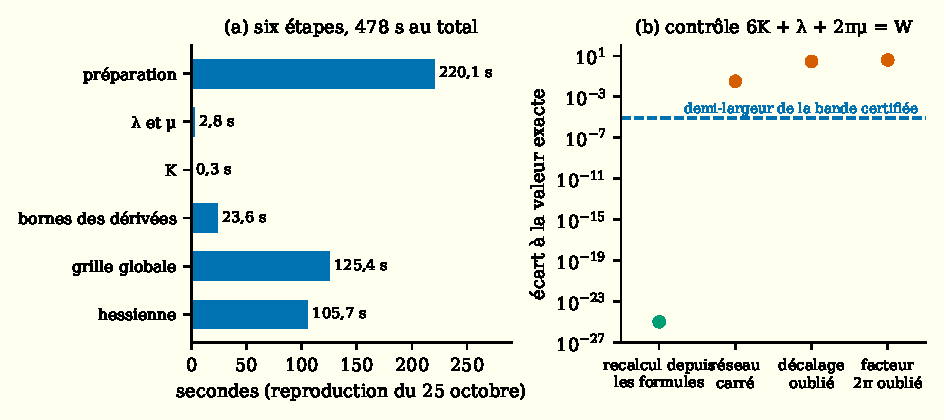
\includegraphics[width=\linewidth]{figures/c13_reproduction}
\caption{(a) Durée des six étapes lors de la reproduction. (b) Le recalcul tombe dans la bande certifiée ; les contrôles faux en sortent.}
\end{figure}
